\documentclass[11pt,a4paper,oneside]{article}


\usepackage[T2A]{fontenc}
\usepackage[utf8]{inputenc}
\usepackage[english,russian]{babel}
\usepackage[russian]{olymp}
\usepackage{graphics}
\usepackage{wrapfig}
\usepackage{amsmath}
\usepackage{amssymb}
\usepackage{epigraph}
\usepackage{graphicx}


\newcommand{\qo}{\textquotesingle}
\newcommand{\qq}{\textquotesingle~}

\contest{ACM ICPC Kyrgyzstan Subregional 2015}{Бишкек}{1 ноября 2015 года}    

\binoppenalty=10000
\relpenalty=10000
\exhyphenpenalty=10000

\renewcommand{\t}{\texttt}

\createsection{\Note}{Примечание}

\renewcommand{\defaultmemorylimit}{256 мегабайт}

\begin{document}

\begin{problem}{Задача I. Ломаная}{1 секунда}{32 мегабайта}

В пространстве даны четыре различных точки с целочисленными координатами, которые представляют ломаную линию из трех звеньев длины единица.

Необходимо распознать и вывести одну из букв, показанных на рисунке 1.
Если ломаная не соответствует ни одной из указанных букв (например, если точки ломаной не лежат в одной плоскости), то вывести слово "Unknown" \hspace{0.3cm} без кавычек.



\begin{figure}[ht]
\centering
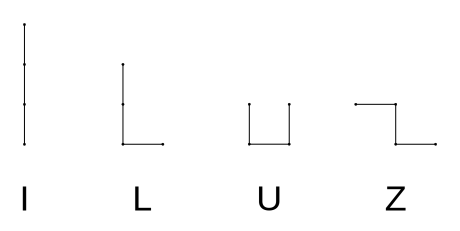
\includegraphics[width=0.4\textwidth]{letters.pdf}
\caption{Буквы для распознавания}
\end{figure}



\InputFile
Четыре строки (все – различные). 
В каждой строке три целых числа в диапазоне 1..9, 
разделенные одинарными пробелами -- координаты точки в пространстве. 
Между каждыми двумя соседними строками разница в единицу 
по одной из координат (правильность исходных данных проверять не нужно). 


\OutputFile
Вывести одну заглавную латинскую букву, или слово "Unknown" \hspace{0.1cm} без кавычек, как указано в задаче.

\Examples

\begin{example}%
\exmp{
1 1 1
1 1 2
1 1 3
1 1 4
}{
I
}%
\exmp{
5 5 5
6 5 5
6 6 5
5 6 5
}{
U
}%
\end{example}



\vspace{1.0cm}
\hfill \textit{Автор задачи: Панков П.C.}
\medskip\noindent




\end{problem}


\end{document}
%%% Local Variables:
%%% mode: latex
%%% TeX-master: t
%%% End:
